There are three decompositions that are used extensively in this thesis: The QR-decomposition, the Singular Value Decomposition, and the Polar Decomposition. All three decompositions are matrix decompositions but can be applied to tensors as well by first grouping indices and reshaping to a matrix, applying the decomposition, and reshaping the result back to the original bond dimensions. \par
The \textit{reduced QR-decomposition} of a matrix $\bm{A} \in \mathbb{C}^{n\times m}$ is the decomposition
\begin{equation}
	\label{eq:QR_decomposition_general}
	\bm{A} = \bm{Q}\bm{R},
\end{equation}
where $\bm{Q}\in\mathbb{C}^{n\times k}$ is an isometry, $\bm{R}\in\mathbb{C}^{k\times m}$ is an upper triangular matrix and $k \coloneqq \min(n, m)$. The computational complexity of the QR decomposition scales as
\begin{equation}
	\label{eq:QR_decomposition_complexity}
	\mathcal{O}\left(n\cdot m\cdot\min(n, m)\right).
\end{equation}
A diagrammatic depiction of the QR decomposition \eqref{eq:QR_decomposition_general} is drawn in figure \figref{fig:tensor_decomposition_diagrams}(a). \par
The \textit{Singular Value Decomposition} (SVD) of a matrix $\bm{A} \in \mathbb{C}^{n\times m}$ is the decomposition
\begin{equation}
	\label{eq:SVD_general}
	\bm{A} = \bm{U}\bm{S}\bm{V}^\dagger,
\end{equation}
where $\bm{U}\in\mathbb{C}^{n\times k}$ and $\bm{V}\in\mathbb{C}^{m\times k}$ are isometries, $\bm{S}\in\mathbb{R}^{k\times k}$ is a diagonal real matrix of \textit{singular values}, and $k \coloneqq \min(n, m)$. The computational complexity of the SVD is the same as for the QR decomposition \eqref{eq:QR_decomposition_complexity}. However, while the scaling is the same, the prefactors are lower for the QR decomposition in most implementations, meaning that the QR decomposition is faster in practice. Moreover, in contrast to the SVD, the QR decomposition allows for highly efficient implementations on graphics processing units (GPUs), which enables decompositions of large matrices to be carried out significantly faster and more power efficiently. Thus, whenever the singular values are not needed, the QR decomposition is preferred over the SVD. Figure \figref{fig:tensor_decomposition_diagrams} shows a tensor network diagram of the SVD \eqref{eq:SVD_general}. \par
An important property of the SVD is that it can be used to approximate a matrix $\bm{A}$ by a matrix $\tilde{\bm{A}}$ of lower rank $\chi < \min(m, n)$. This \textit{truncated SVD} can be performed by keeping only the largest $\chi < k$ singular values and omitting the corresponding columns of $\bm{U}$ and $\bm{V}$:
\begin{equation}
	\label{eq:truncated_SVD_general}
	\bm{A} \approx \tilde{\bm{A}} = \tilde{\bm{U}}\tilde{\bm{S}}\tilde{\bm{V}},
\end{equation}
with isometries $\tilde{\bm{U}}\in\mathbb{C}^{n\times\chi}$, $\tilde{\bm{V}}\in\mathbb{C}^{m\times\chi}$ and real diagonal matrix $\tilde{\bm{S}}\in\mathbb{C}^{\chi\times\chi}$. It can be shown \cite{cite:eckart_young_theorem} that the truncated SVD minimizes the distance $\lVert \bm{A} - \bm{\tilde{A}} \rVert_\text{F}$ between $\bm{A}$ and $\tilde{\bm{A}}$ under the constraint $\text{rank}(\tilde{\bm{A}}) = \chi$. The truncated SVD is frequently used in tensor network algorithms to truncate tensors to a maximum bond dimension $\chi_\text{max}$. \par
The \textit{polar decomposition} of a matrix $\bm{A} \in \mathbb{C}^{n\times m}$ is the decomposition
\begin{equation}
	\label{eq:polar_decomposition_general}
	\bm{A} = \bm{W}\bm{P},
\end{equation}
where $\bm{W}\in\mathbb{C}^{m\times n}$ is an isometry and $\bm{P}\in\mathbb{C}^{n\times n}$ is positive-definite and hermitean. The polar decomposition is related to the SVD $\bm{A} = \bm{U}\bm{S}\bm{V}$ by
\begin{equation}
	\label{eq:polar_decomposition_connection_to_svd}
	\bm{W} = \bm{U}\bm{V}^\dagger, \quad \bm{P} = \bm{V}\bm{S}\bm{V}^\dagger.
\end{equation}
The computational complexity of the polar decomposition is the same as for the QR decomposition and SVD \eqref{eq:QR_decomposition_complexity}. The polar decomposition \eqref{eq:polar_decomposition_general} is depicted diagrammatically in figure \figref{fig:tensor_decomposition_diagrams} One can show \todo{prove in appendix?} that the $\bm{W}$ factor of the polar decomposition is the isometry "closest" to the matrix $\bm{A}$, i.e. the isometry that minimizes the distance $\lVert\bm{A}-\bm{W}\rVert_\text{F}$. Thus, the polar decomposition is often used in isometric tensor network algorithms to "isometrize" tensors.
\begin{figure}
	\centering
	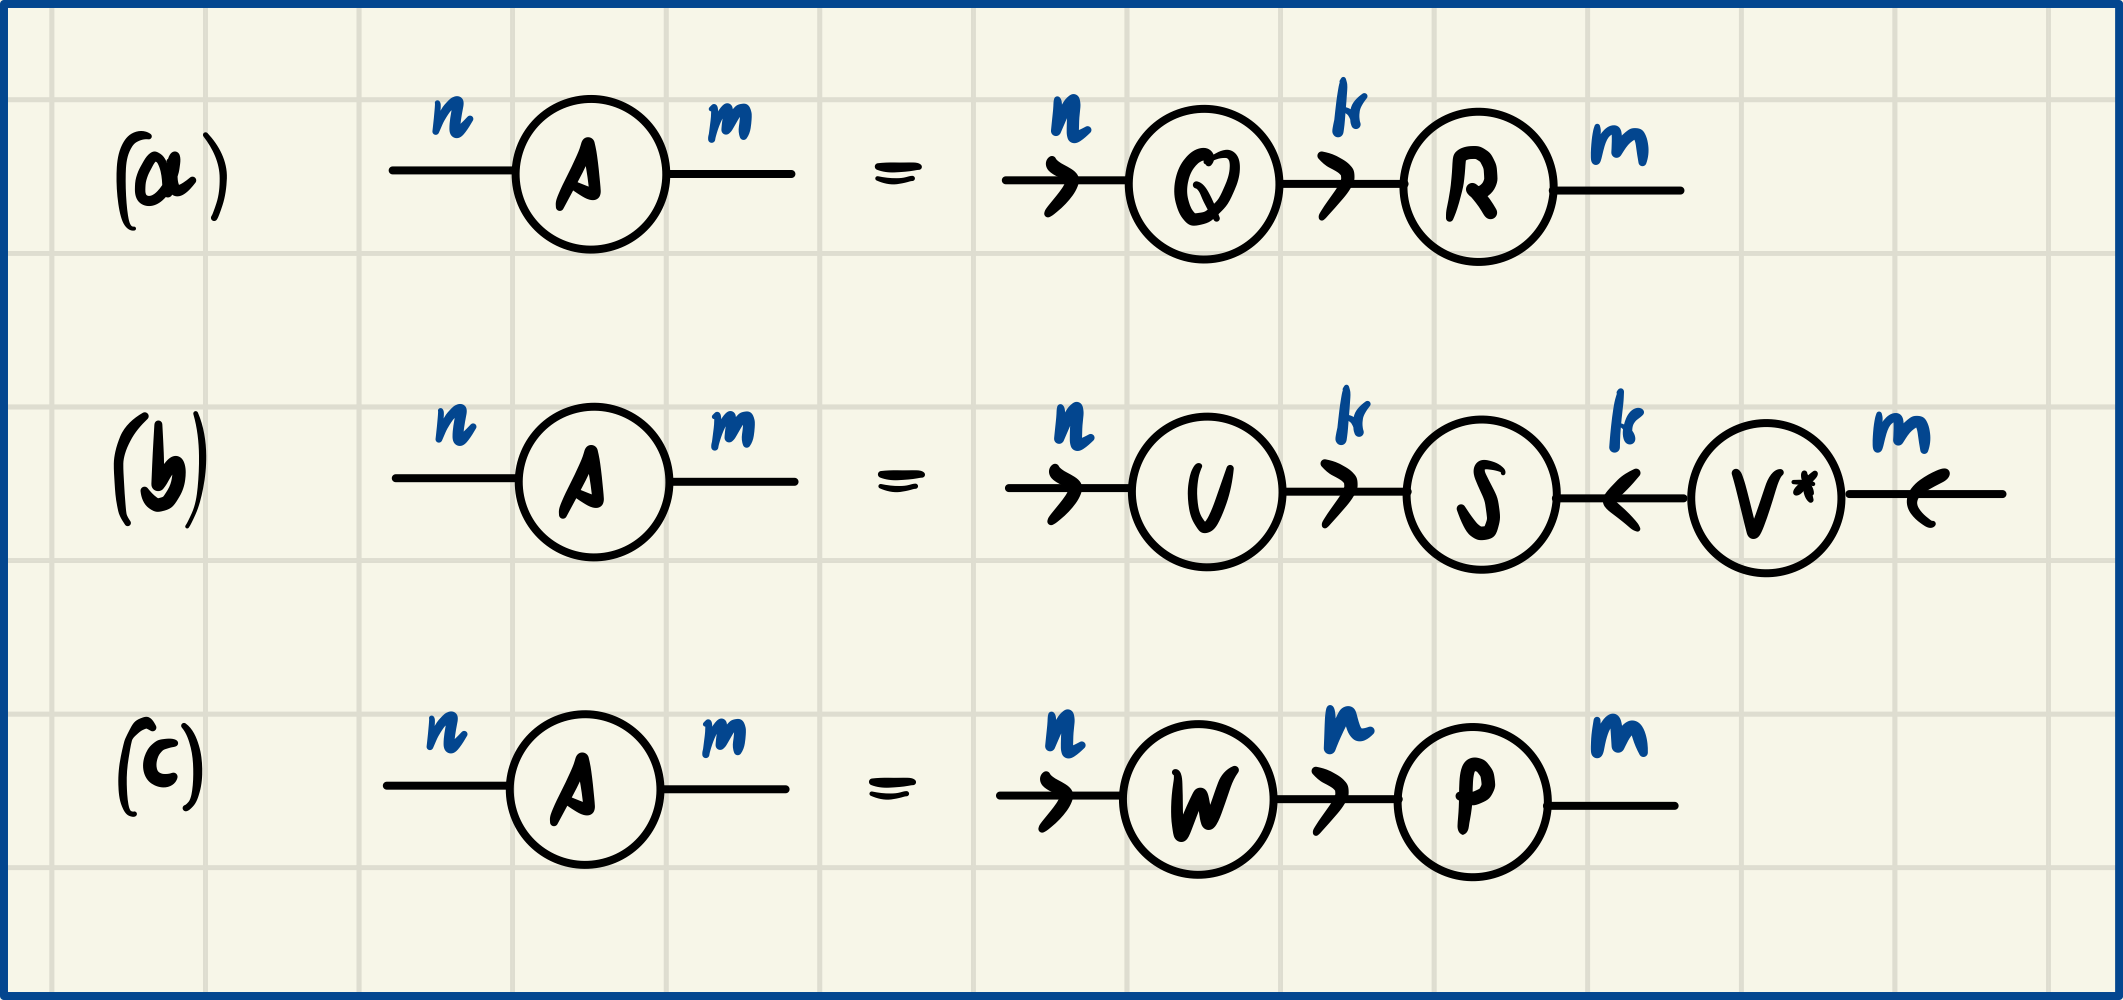
\includegraphics[width=0.8\textwidth]{figures/Tensor_Networks/tensor_decomposition_diagrams.jpeg}
	\caption{Different tensor decompositions are shown in tensor network diagram notation. The indices are decorated with bond dimensions. (a) QR decomposition \eqref{eq:QR_decomposition_general}. (b) Singular Value Decomposition \eqref{eq:SVD_general}. (c) Polar decomposition \eqref{eq:polar_decomposition_general}.}
	\label{fig:tensor_decomposition_diagrams}
\end{figure}